% Created 2024-10-16 śro 21:35
% Intended LaTeX compiler: pdflatex
\documentclass[../main.tex]{subfiles}

% \usepackage[a4paper, margin=3cm]{geometry}
% \usepackage{amssymb} // not working

\usepackage[T1]{fontenc}
\usepackage[utf8]{inputenc}
\usepackage{graphicx}
\usepackage{longtable}
\usepackage{wrapfig}
\usepackage{rotating}
\usepackage[normalem]{ulem}
\usepackage{amsmath}
\usepackage{capt-of}
\usepackage{hyperref}
\usepackage{siunitx}
\usepackage{float}
\usepackage[polish]{babel}

\graphicspath{{../}}
\author{Wojciech Paderewski}
\date{\today}
\title{Esp32}
\hypersetup{
 pdfauthor={Wojciech Paderewski},
 pdftitle={Esp32},
 pdfkeywords={},
 pdfsubject={},
 pdflang={Polish}}

\begin{document}

ESP32-S3 to mikrokontroler firmy Espressif Systems, który jest następcą popularnego ESP32.
Jednego z najpopularniejszych mikrokontrolerów z modułem WiFi wykorzystanego w wielu projektach IoT.
Układ ten posiada następujące cechy odczytane z karty katalogowej \cite{st:esp32}:

\begin{itemize}
\item 2 rdzenie Xtensa LX7 o taktowaniu 240 MHz
\item 2,4 GHz WiFi 4 (802.11 b/g/n)
\item Bluetooth 5.0 LE
\item dwa 12-bitowe przetworniki ADC do 20 kanałów
\item 14 pinów do obsługi dotykowego ekranu
\item 45 programowalnych GPIO - część z nich ma specjalne funkcje
\item kontroler USB/JTAG
\item ROM: 384 KB
\item SRAM: 512 KB
\item Wbudowany moduł RTC
\end{itemize}
\subsection{Moduł RTC}

RTC (Real Time Clock) to moduł zegara czasu rzeczywistego, który pozwala na śledzenie aktualnego czasu, daty oraz dnia tygodnia.
Moduł RTC w ESP32-S3 wykorzystuje 16 kB pamięci SRAM, co oznacza, że nie może on przechowywać daty i czasu w przypadku braku zasilania.

Sam moduł zegara czasu rzeczywistego nie jest bardzo dokładny; dlatego zaleca się synchronizację czasu z zewnętrznym serwerem.
Istnieje wiele bibliotek do realizacji tego zadania z wykorzystaniem Arduino Framework.
\subsection{GPIO}
Układ posiada wiele wyprowadzeń wejścia/wyjścia ogólnego przeznaczenia (GPIO). Nie posiada on dedykowanych pinów do obsługi interfejsów takich jak I2C, można 
je skonfigurować na dowolnych pinach GPIO. Generacja sygnałów PWM jest również możliwa na większości wyprowadzeń. Posiada on również 20 pinów które mogą
obsługiwać wejście analogowe. Rozkład pinów mikrokontrolera ESP32-S3 przedstawiono na \ref{fig:esp32}.


\begin{figure}[H]
  \centering
  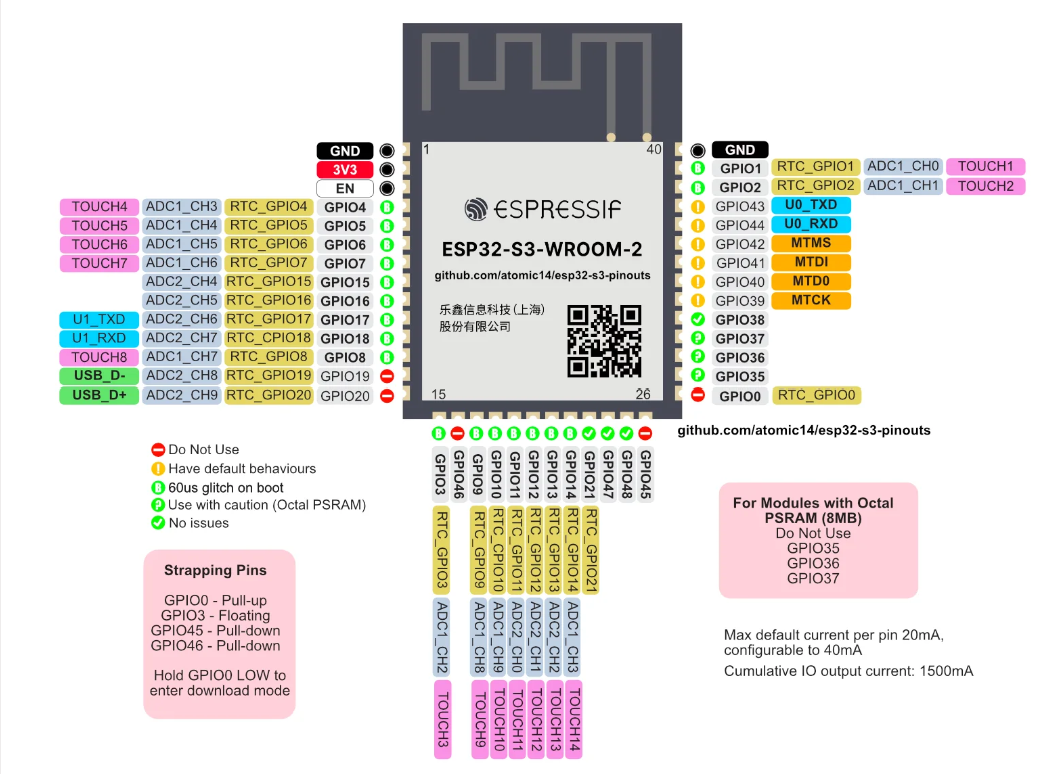
\includegraphics[width=1\textwidth]{Esp32.png}
  \caption{Rozkład pinów mikrokontrolera ESP32-S3 \cite{st:esp32-pin}}
  \label{fig:esp32}
\end{figure}

\subsection{Kontroler USB/JTAG}
ESP32-S3 posiada wbudowany kontroler USB/JTAG, pozwalający programować układ bez użycia zewnętrznego programatora.
Wyprowadzenia do programowania układu za pośrednictwem interfejsu USB to GPIO19(D-) oraz GPIO20(D+).
Istnieje również możliwość programowania układu za pomocą protokołu UART korzystając z pinów GPIO1(TX) oraz GPIO3(RX).


\subsection{Zasilanie}
Według dokumentacji producenta, ESP32-S3 może być zasilany napięciem od \SI{3}{\volt} do \SI{3.6}{\volt}, zalecane napięcie zasilania to \SI{3.3}{\volt}.
Jego maksymalny pobór prądu wynosi \SI{340}{\milli\ampere}, jednak w praktyce jest on znacznie mniejszy, zależy to od wykorzystywanych funkcji i peryferiów.

Układ można wprowadzić w dwa tryby uśpienia:
\begin{itemize}
\item Light Sleep - pobór prądu wynosi około \SI{240}{\micro\ampere}, w tym odłączany jest moduł WiFi a wszystkie piny GPIO są w stanie wysokiej impedancji.
\item Deep Sleep - pobór prądu wynosi około \SI{8}{\micro\ampere}, jedynie zasilany jest moduł zegara czasu rzeczywistego, wszystkie inne funkcje są wyłączone.
\end{itemize}

\subsubsection{Środowisko programistyczne}
\label{sec:srodowisko_programistyczne}
ESP32-S3 jest na tyle rozbudowanym mikrokontrolerem, że wymaga pozwala on na programowanie w wielu językach programowania, takich jak C, C++, MicroPython, Lua oraz Rust.
najpopularniejszym językiem programowania dla ESP32-S3 jest C++, jest on bardzo wydajny, a przy tym pozwala na wysokopoziomowe programowanie, 
co znacząco przyspiesza pisanie kodu oraz jego czytelność, również dla tego języka występuje najwięcej bibliotek i przykładów.

W przypadku ESP32-S3 najczęściej wykorzystuje się Arduino Framework, które jest najbardziej popularnym rozwiązaniem dla mikrokontrolerów ESP32. Można również korzystać z ESP-IDF,
które jest oficjalnym środowiskiem programistycznym dla mikrokontrolerów rodziny ESP32, ale jest ono bardziej skomplikowane i wymaga więcej czasu na naukę. Dwoma
najpopularniejszymi środowiskami programistycznymi dla ESP32-S3 są PlatformIO oraz Arduino IDE.

\end{document}
